
% Due thursday

\documentclass{article}

\usepackage[utf8]{inputenc}

\usepackage{amsmath, bm}
\usepackage{graphicx}
\usepackage{amssymb}
\usepackage{float}
\usepackage{caption}
\usepackage{subcaption}
\usepackage{hyperref}
\usepackage{tikz}
\usepackage{layout}

\usepackage[margin=1in]{geometry}
\usepackage{listings}
\usepackage{xcolor}
\usepackage{color, colortbl}
\usepackage{textgreek}
\usepackage{mathrsfs}
\usepackage{savetrees}


\setlength{\parskip}{\baselineskip}%
\setlength{\parindent}{0pt}%
\linespread{0.9}


\definecolor{codegreen}{rgb}{0,0.6,0}
\definecolor{codegray}{rgb}{0.5,0.5,0.5}
\definecolor{codepurple}{rgb}{0.58,0,0.82}
\definecolor{backcolour}{rgb}{0.95,0.95,0.92}

\lstdefinestyle{mystyle}{
    backgroundcolor=\color{backcolour},   
    commentstyle=\color{codegreen},
    keywordstyle=\color{magenta},
    numberstyle=\tiny\color{codegray},
    stringstyle=\color{codepurple},
    basicstyle=\ttfamily\footnotesize,
    breakatwhitespace=false,         
    breaklines=true,                 
    captionpos=b,                    
    keepspaces=true,                 
    numbers=left,                    
    numbersep=5pt,                  
    showspaces=false,                
    showstringspaces=false,
    showtabs=false,                  
    tabsize=2
}

\lstset{style=mystyle}



\begin{document}

\title{GA3: Heat Exchanger Performance Report}
\author{lwp26 - Group E}
\date{May 2024}
\maketitle 

\section{Introduction}

The performance of various heat exchanger geometries can be analysed using the software previously developed.
The resulting heat transfer rate $\dot{Q}$ depends on many variables, and experimental data used to calibrate the software.
However, the confidence in the software's predictions is limited by uncertainty in input variables and methods used to calibrate the software from limited experimental data.
This report will analyse the uncertainty in the software's predictions and compare the performance of various groups heat exchanger designs.
% group C manifold

\section{Uncertainty Analysis}
The heat transfer rate is a function of geometry, operating conditions and compressor characteristics defined below.
\begin{equation}
    \dot{Q} = f(L_\text{tube}, Y, B, T_{1in}, T_{2in}, \dot{m}_1(\Delta P_1), \dot{m}_2(\Delta P_2)) = f(x_1, \; \dots \; x_i \; \dots \; , x_N, \dot{m}_1(\Delta P_1), \dot{m}_2(\Delta P_2))
\end{equation}
The relative uncertainty of $\dot{Q}$ due to absolute uncertainty $\delta x_i$ is found numerically by a central difference method:
\begin{equation}
    u_i(\dot{Q}) \approx \frac{1}{\dot{Q}}\left|\frac{\partial \dot{Q}}{\partial x_i} \delta x_i \right| \approx \frac{ \left| \dot{Q}(x_i + \delta x_i) - \dot{Q}(x_i - \delta x_i) \right|}{2\dot{Q}(x_i)} \label{eq:central_difference} \quad \text{and} \quad u(\dot{Q}) = \sqrt{\sum_{i=1}^N u_i(\dot{Q})^2}
\end{equation}
The uncertainty in compressor characteristics is handled by applying the uncertainty band to pressures at all operating points \ref{fig:compressor_uncertainty}.
An initial test was performed to determine the sensitivity of $\dot{Q}$ to baffle spacing, pitch and length.
The absolute uncertainty in baffle spacing, pitch and length is taken to be 1mm.
This represents a high relative uncertainty in the pitch due to the empirical method used in the software.
The relative uncertainty in calculated $\dot{Q}$ was found to be 0.00546\%, 0.58286\% and 0.11430\% for baffle spacing, pitch and length respectively.
This shows that an uncertainty in baffle spacing has negligible effect and is not considered in further analysis.
For all 2024 designs the number of tubes and baffles are equal in each of the designs cross sections.

\subsection{Special Cases}

Group C have a unique manifold for their hot section flow and so have a reduced pressure rise across the hot section.
The pressure loss coefficient is not known and so the nozzle loss coefficient was underestimated to be 0.
The expansion and constriction losses were taken to be the same as other groups 

\subsection{Uncertainty of Inputs}

To perform further uncertainty analysis the uncertainty in input variables must be determined.
For length the uncertainty can be estimated from CAD drawings and manufacturing processes.
The uncertainty in the pitch is harder to determine.

Given that the CAD drawings are available, it makes sense to define a true average pitch and compare this to the calculated pitch to determine the uncertainty.
The true average pitch is defined as the average edge length of a network spanning a given hot section.
For all designs in 2024 the hot sections are circularly symmetric and so the average pitch is the same for all hot sections.
The absolute uncertainty in the pitch is then taken to be the maximum difference between the calculated and true average pitch.

\begin{minipage}[t]{0.29\textwidth}
    \centering
    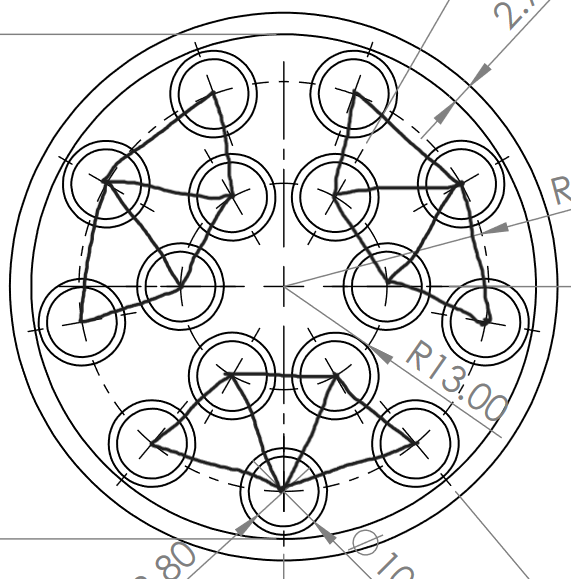
\includegraphics[width=0.8\textwidth]{tube_network.png}
    \captionof{figure}{Three tube networks in our heat exchanger design}
    \label{fig:tube_network}
\end{minipage}
\begin{minipage}[t]{0.69\textwidth}
    \centering
    \begin{tabular}{c|c|c}
        Design & Calculated Pitch & True Average Pitch \\
        & (mm) & (mm) \\
        \hline
        A & 16.33 & 12.00 \\
        B & 16.33 & 15.41 \\
        C & 16.33 & 14.67 \\
        D & 15.21 & 12.00 \\
        E & 14.49 & 15.13 \\
    \end{tabular}
    \captionof{table}{Pitch Comparison}
    \label{tab:pitch_comparison}
\end{minipage}

The uncertainty in the compressor characteristics is assumed to be 5\% as shown below in figure \ref{fig:compressor_uncertainty}.
The uncertainty in $\dot{Q}$ was found by calculating the same central difference method at 5\% higher and lower pressure characteristic pressure curves.
These are shown by the upper and lower lines of the shaded regions in figure \ref{fig:compressor_uncertainty}

\begin{figure}[H]
    \centering
    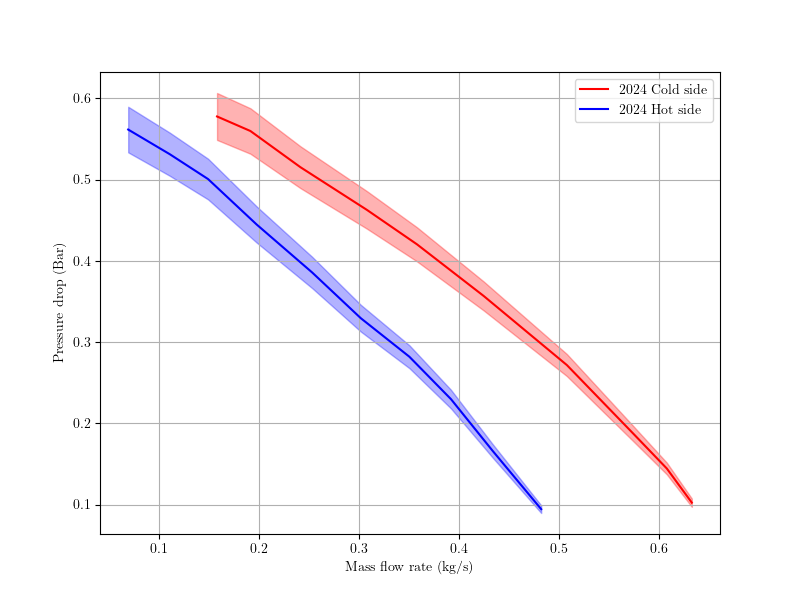
\includegraphics[width=0.6\textwidth]{compressor_characteristics.png}
    \caption{Assumed 5\% uncertainty in compressor characteristics}
    \label{fig:compressor_uncertainty}
\end{figure}

\subsection{Uncertainty of Outputs}
Corrections from available experimental data were applied to the pressure calculations to improve the accuracy Kerns method.
The uncertainty in mass flow from these corrections is not considered in this short report.
A correction was also applied to the final $\dot{Q}$ value as it had a strong correlation coefficient.
Uncertainty in the uncorrected $\dot{Q}$ was estimated for each variable by the same central difference method in equation \ref{eq:central_difference}.
These values are shown for each design in the table \ref{tab:uncorrected_uncertainty} below, along with the overall propagated uncertainty.


\begin{table}[h!]
    \centering
    \begin{tabular}{c|c|c|c|c|c|c|c|c}

        Group & $u_Y(\dot{Q})$ & $u_L(\dot{Q})$ & $u_{T_\text{1in}}(\dot{Q})$ & $u_{T_\text{2in}}(\dot{Q})$ & $u_\text{cold}(\dot{Q})$ & $u_\text{hot}(\dot{Q})$ & $u_\text{unc}(\dot{Q})$ & $u_\text{cor}(\dot{Q})$\\
        & (\%) & (\%) & (\%) & (\%) & (\%) & (\%) & (\%) & (\%) \\
    \hline
    Group-A & 2.384050     & 0.119312      & 1.348202    & 1.348202    & 0.718815    & 1.257291   & 3.380932 & 12.30      \\
    Group-B & 2.307477     & 0.127439      & 1.322163    & 1.322163    & 0.690370    & 1.243790   & 3.295534 & 12.35    \\
    Group-C & 2.437940     & 0.116954      & 1.367768    & 1.367768    & 0.726736    & 1.266629   & 3.439666 & 12.31     \\
    Group-D & 3.174105     & 0.132264      & 1.318523    & 1.318523    & 0.714964    & 1.235442   & 3.950561 & 12.69     \\
    Group-E & 3.860030     & 0.137442      & 1.371735    & 1.371735    & 0.735290    & 1.162906   & 4.535972 & 12.84    \\
    \end{tabular}
    \caption{Table of u\_Qdot values for different groups}
    \label{tab:uncorrected_uncertainty}
\end{table}

The correction applied to $\dot{Q}$ was based on a limited set of 2022 and 2023 data.
The uncertainty in the slope and intercept coefficients for this correction was estimated using a t-distribution with a 90\% confidence level.
This is displayed with the uncorrected uncertainty below in figure \ref{fig:uncertainty_regions}.

\begin{figure}[H]
    \centering
    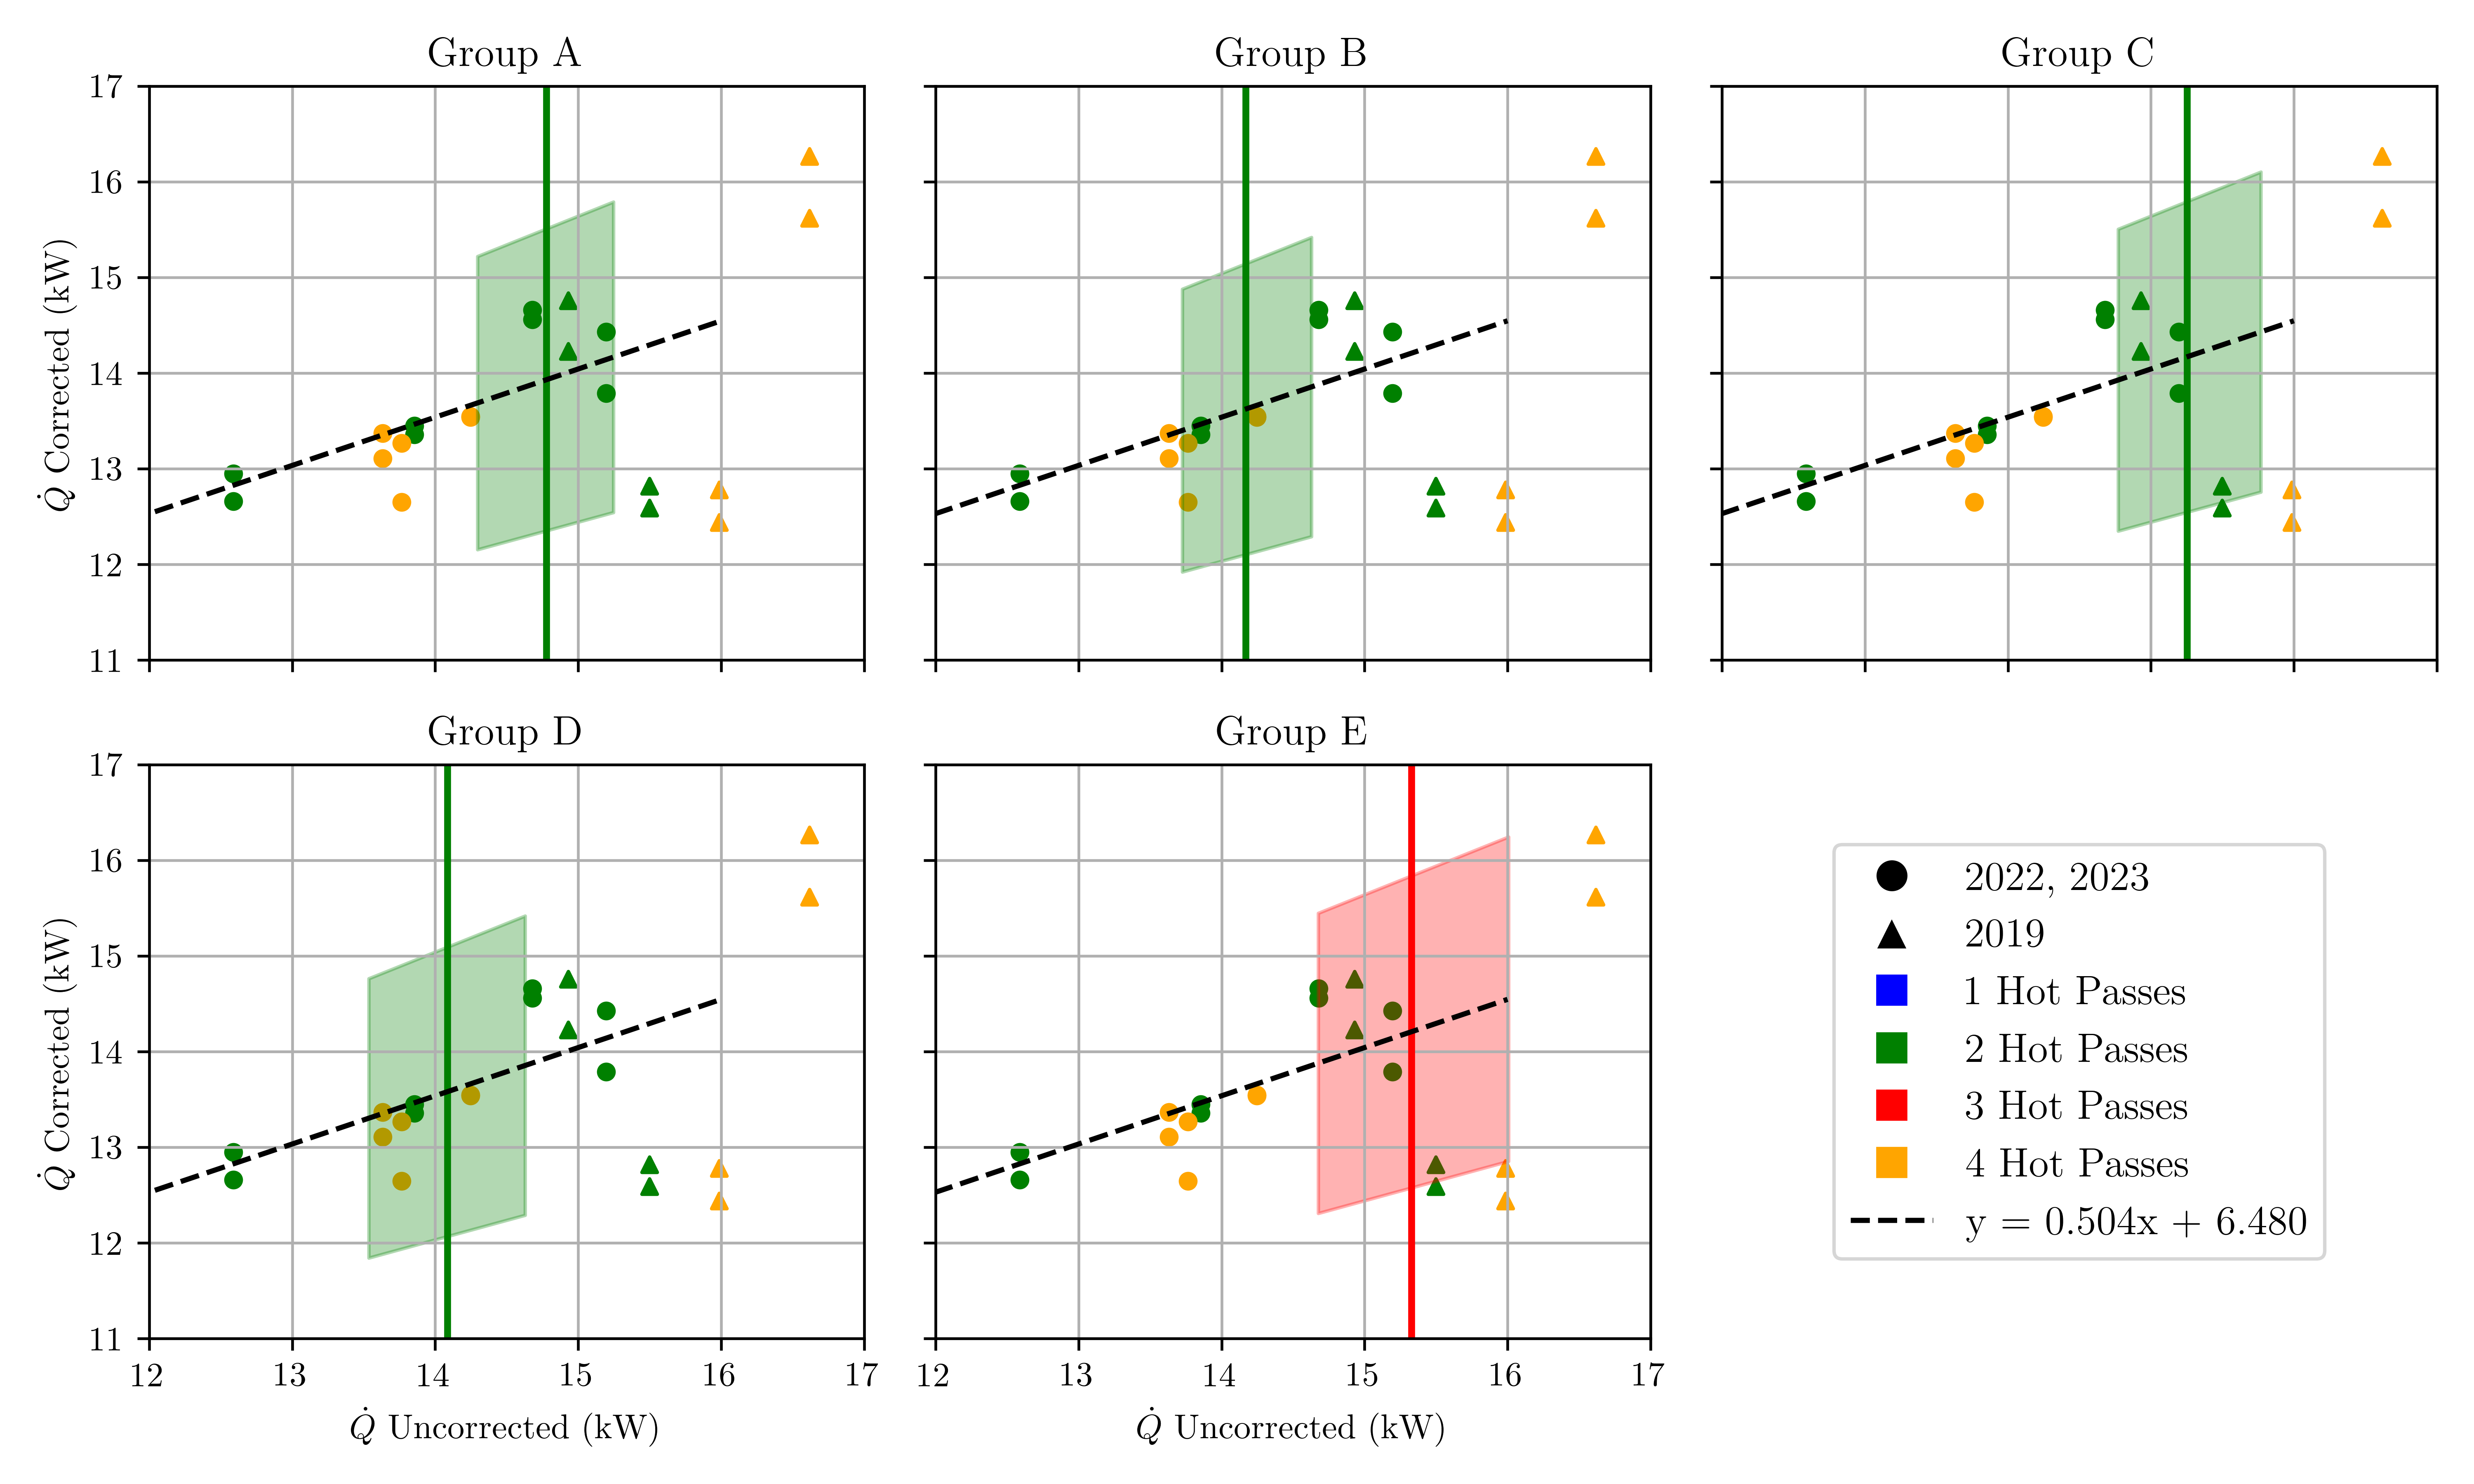
\includegraphics[width=0.99\textwidth]{Qdot_uncertainty_bands.png}
    \caption{$\dot{Q}$ Uncertainty Regions for 2024 Designs given uncorrected \ref{tab:uncorrected_uncertainty}}
    \label{fig:uncertainty_regions}
\end{figure}

This shows a significant uncertainty in the corrected $\dot{Q}$ value for all designs. Comparisons between designs are difficult due to the large uncertainty in the corrected $\dot{Q}$ value.
The uncertainty in our, group E, design is slightly higher than other groups due to our high tube count and high relative uncertainty in calculated pitch.
The impact this has on $\dot{Q}$ can be seen in the table \ref{tab:uncorrected_uncertainty}.
Variables that affect $\dot{Q}$ the most are hot pressure characteristics and both hot and cold inlet temperatures.

\section{Performance Degradation}

Fouling is a common issue in heat exchangers, leading to a reduction in heat transfer coefficient and reduction in tube areas.
This can be due to a variety of mechanisms depending on the fluid, geometry and operating conditions.
For feedwater heaters the most common fouling mechanisms are deposition of iron oxides and inorganic salts \cite{HeatTransfer}.
This is often modelled by an empirical fouling factor, which acts as additional thermal resistance \cite{HeatTransfer}.
For shell and tube heat exchangers, this fouling factor has been found to increase over time \cite{fouling}.
We will only consider a constant fouling factor of $R_f = 0.00174$. The total fouling factor \cite{HE_design} is defined for both sides of the pipe as:
\begin{equation}
    R_{Tf} = R_f \left( 1 + \frac{d_o}{d_i} \right)
\end{equation}

\subsection{Performance Comparison}

\begin{figure}[H]
    \centering
    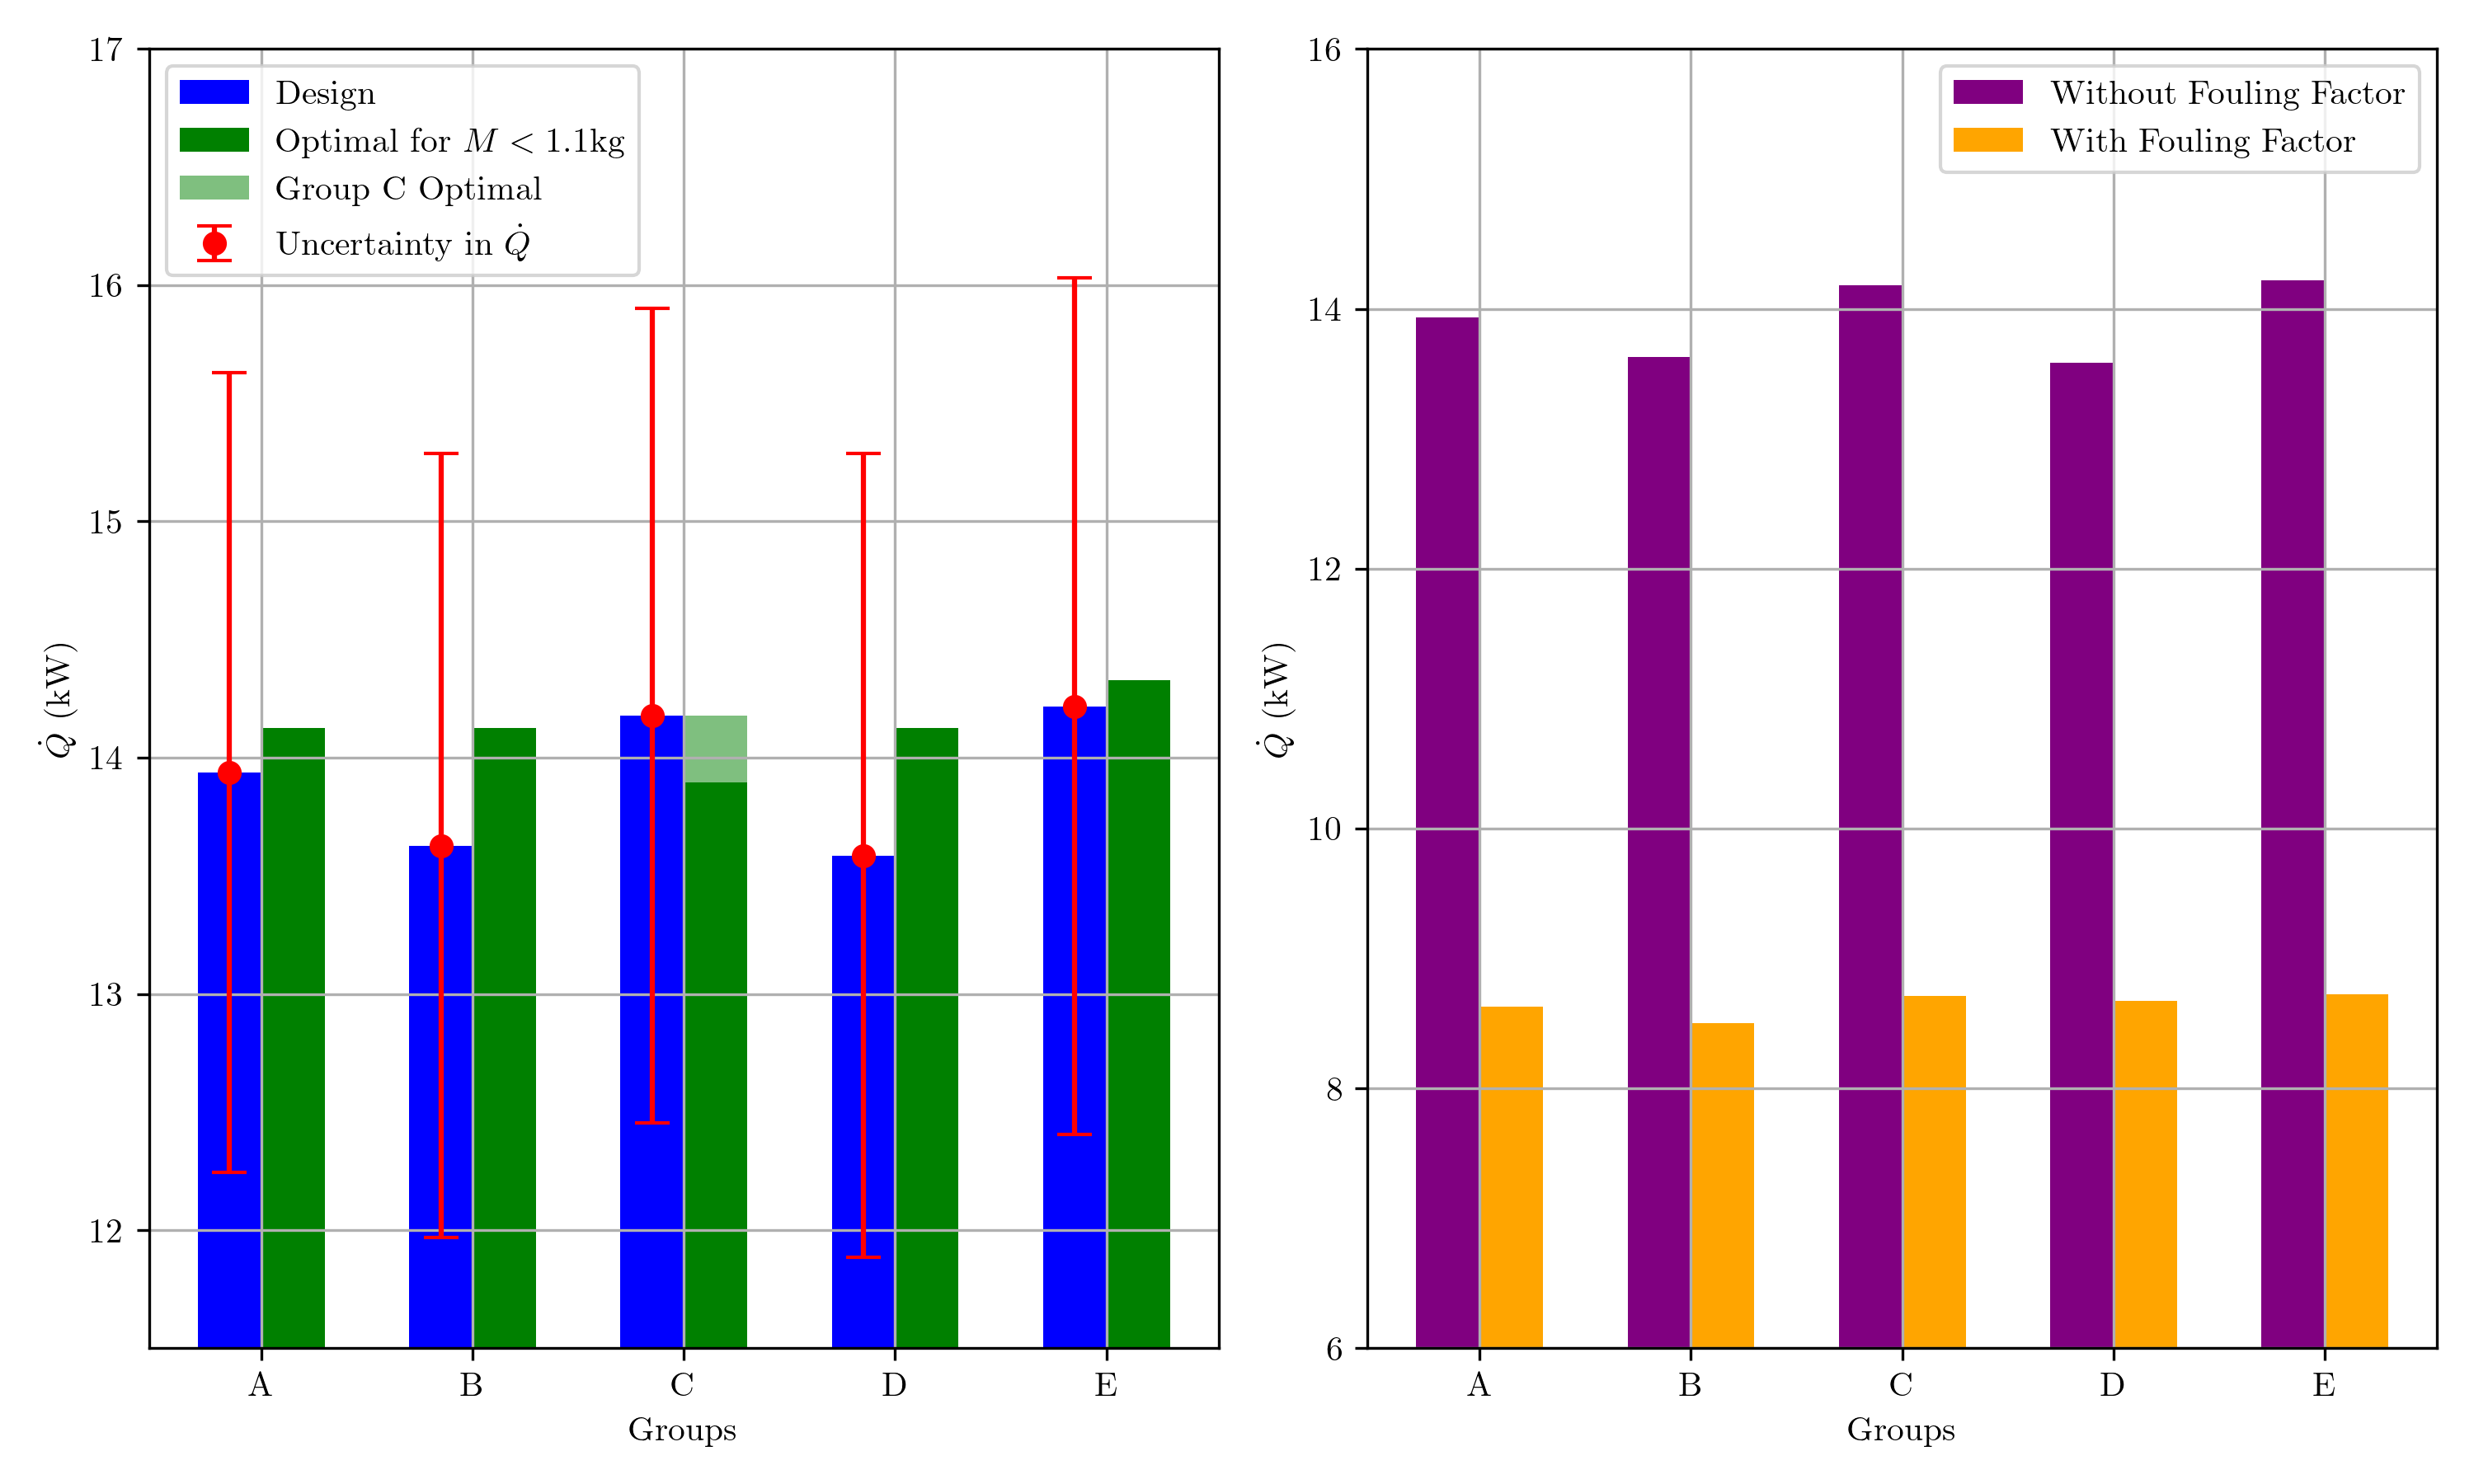
\includegraphics[width=0.8\textwidth]{2024comparison.png}
    \caption{2024 Performance Comparison}
    \label{fig:2024_performance}
\end{figure}

The performance of the 2024 designs is shown in figure \ref{fig:2024_performance}.
With little confidence, our software predicts that our design will perform the best out of all groups.
It can also be seen that despite small manufacturing modifications made to our design, it is still close to the optimal found.
Group C's design was predicted to come 2nd with a heat transfer 0.28\% below our design.
Their design was calculated to be much heavier at 1.145 kg, which does not accurately include the weight of the manifold.
A seperate optimisation was performed with a relaxed mass constraint, which agreed that group C's design was the closest to optimal.
In third place was group A, with a heat transfer 1.97\% below our design. This was 1.34 \% below predicted optimal for their configuration.
Groups B and D were predicted at 4th and 5th place respectively, with heat transfers 4.15\% and 4.44\% below our design.
These were also 3.53\% and 3.82\% below predicted optimal for their configurations.

\begin{thebibliography}{9}

    %Endres, SC, Sandrock, C, Focke, WW (2018) “A simplicial homology algorithm for lipschitz optimisation”, Journal of Global Optimization.
    
      \bibitem{handout}
      J. V. Taylor and J. C. Massey
      \emph{GA3 Heat Exchanger Handout}
      University of Cambridge,
      2024.
    
      \bibitem{HeatTransfer}
      Holman J. P.
      \emph{Heat Transfer. 10th ed.}
      McGraw-Hill,
      2010.

      \bibitem{HE_design}
        Sadik Kakac, Hongtan Liu, Anchasa Pramuanjaroenkij,
        \emph{Heat Exchangers: Selection, Rating, and Thermal Design, Third Edition}
        CRC Press,
        2012.

      \bibitem{fouling}
      M. Ratel, Y. Kapoor, Z. Anxionnaz-Minvielle, L Seminel, B. Vinet
      \emph{INVESTIGATON OF FOULING RATES IN A HEAT EXCHANGER USING AN INNOVATIVE FOULING RIG}
      International Conference on Heat Exchanger Fouling and Cleaning
      2013

\end{thebibliography}


\end{document}